\documentclass[12pt,a4paper]{article}

% ─── PACKAGES ────────────────────────────────────────────────────────
\usepackage[margin=1in]{geometry}
\usepackage{graphicx}
\usepackage{booktabs}
\usepackage{hyperref}
\usepackage{enumitem}
\usepackage{tabularx}
\usepackage{longtable}
\usepackage{tikz}
\usetikzlibrary{positioning, arrows.meta, shapes.multipart, calc}
\usepackage{fancyhdr}
\usepackage{titlesec}

% ─── SETTINGS ────────────────────────────────────────────────────────
\hypersetup{colorlinks=true, linkcolor=blue, urlcolor=blue}
\pagestyle{fancy}
\fancyhf{}
\rhead{Placement Portal Application}
\lhead{Project Report}
\cfoot{\thepage}
\setlength{\parindent}{0pt}
\setlength{\parskip}{6pt}
\titlespacing*{\section}{0pt}{12pt}{6pt}
\titlespacing*{\subsection}{0pt}{8pt}{4pt}

% ═════════════════════════════════════════════════════════════════════
\begin{document}

% ─── TITLE PAGE / HEADER ────────────────────────────────────────────
\begin{center}
    {\LARGE \textbf{Placement Portal Application}} \\[6pt]
    {\large Project Report} \\[12pt]
\end{center}

% ─── 1. STUDENT DETAILS ─────────────────────────────────────────────
\section{Student Details}

\begin{tabularx}{\textwidth}{|l|X|}
\hline
\textbf{Name}           & \textit{[Your Full Name]}        \\ \hline
\textbf{Roll Number}    & \textit{[Your Roll Number]}      \\ \hline
\textbf{Email}          & \textit{[Your Email ID]}         \\ \hline
\textbf{Course}         & \textit{[Your Course Name]}      \\ \hline
\textbf{Batch}          & \textit{[Your Batch / Year]}     \\ \hline
\end{tabularx}

% ─── 2. PROJECT DETAILS ─────────────────────────────────────────────
\section{Project Details}

\subsection{Problem Statement}
Institutes need efficient systems to manage campus recruitment activities involving
companies, students, and placement drives. The goal is to build a \textbf{Placement
Portal Application} that allows Admin (Institute), Company, and Student users to
interact with the system based on their roles --- managing company approvals,
placement drives, student applications, and recruitment outcomes.

\subsection{Approach}
\begin{enumerate}[leftmargin=*]
    \item \textbf{Requirement Analysis:} Identified three roles (Admin, Company, Student)
          and their functionalities as described in the problem statement.
    \item \textbf{Database Design:} Designed 5 relational tables (User, StudentProfile,
          CompanyProfile, PlacementDrive, Application) with proper foreign keys and
          constraints.
    \item \textbf{Backend Development:} Built the Flask application with route controllers
          organized by role (\texttt{auth.py}, \texttt{admin.py}, \texttt{company.py},
          \texttt{student.py}).
    \item \textbf{Frontend Development:} Created Jinja2 templates with Bootstrap 5 for
          responsive UI, organized in subfolders by role.
    \item \textbf{Testing:} Tested all flows --- registration, login, approval workflow,
          drive creation, application, status updates, search, and blacklisting.
\end{enumerate}

% ─── 3. AI/LLM DECLARATION ──────────────────────────────────────────
\section{AI/LLM Declaration}

\begin{tabularx}{\textwidth}{|l|X|}
\hline
\textbf{AI Tool Used}       & Claude (Anthropic)                             \\ \hline
\textbf{Extent of Use}      & Used for code generation, debugging assistance,
                               project structuring, and report template creation. \\ \hline
\textbf{What was AI-generated} & Initial boilerplate code, form definitions,
                               template structure, database model definitions.    \\ \hline
\textbf{What was done manually} & Project architecture decisions, testing all
                               features, customization, understanding the code,
                               video recording, and viva preparation.            \\ \hline
\end{tabularx}

% ─── 4. FRAMEWORKS AND LIBRARIES ────────────────────────────────────
\section{Frameworks and Libraries Used}

\begin{tabularx}{\textwidth}{|l|l|X|}
\hline
\textbf{Library}        & \textbf{Version} & \textbf{Purpose}                    \\ \hline
Flask                   & 3.0.0            & Web application framework           \\ \hline
Flask-SQLAlchemy        & 3.1.1            & ORM for SQLite database             \\ \hline
Flask-Login             & 0.6.3            & User session \& authentication      \\ \hline
Flask-WTF               & 1.2.1            & Form handling with CSRF protection  \\ \hline
WTForms                 & 3.1.1            & Form field definitions \& validation\\ \hline
Werkzeug                & 3.0.1            & Password hashing \& file uploads    \\ \hline
email-validator         & 2.1.0            & Email format validation             \\ \hline
Jinja2                  & (bundled)        & HTML template rendering             \\ \hline
Bootstrap               & 5.3.2            & Responsive CSS framework (CDN)      \\ \hline
SQLite                  & (built-in)       & Lightweight relational database     \\ \hline
\end{tabularx}

% ─── 5. ER DIAGRAM ──────────────────────────────────────────────────
\section{ER Diagram}

\begin{center}
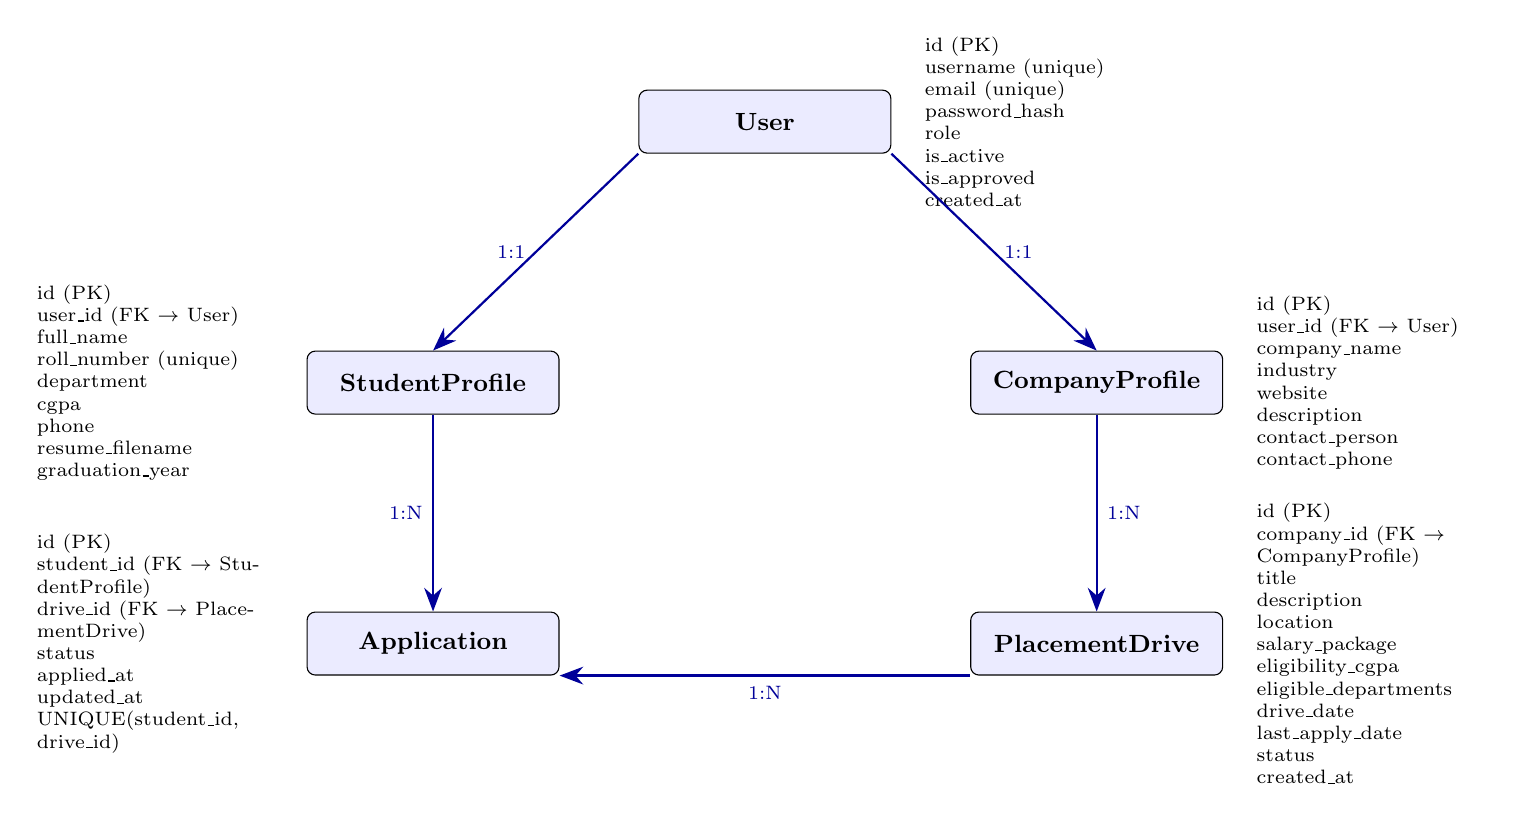
\begin{tikzpicture}[
    entity/.style={rectangle, draw=black, fill=blue!8, minimum width=3.2cm,
                   minimum height=0.8cm, font=\small\bfseries, rounded corners=3pt},
    attr/.style={font=\scriptsize, text width=3cm, align=left},
    rel/.style={-{Stealth[length=3mm]}, thick, blue!60!black},
    node distance=1.5cm and 3.5cm
]

% Entities
\node[entity] (user) {User};
\node[entity, below left=2.5cm and 1cm of user] (student) {StudentProfile};
\node[entity, below right=2.5cm and 1cm of user] (company) {CompanyProfile};
\node[entity, below=2.5cm of company] (drive) {PlacementDrive};
\node[entity, below=2.5cm of student] (app) {Application};

% Attributes
\node[attr, right=0.3cm of user] {id (PK)\\username (unique)\\email (unique)\\password\_hash\\role\\is\_active\\is\_approved\\created\_at};

\node[attr, left=0.3cm of student] {id (PK)\\user\_id (FK $\to$ User)\\full\_name\\roll\_number (unique)\\department\\cgpa\\phone\\resume\_filename\\graduation\_year};

\node[attr, right=0.3cm of company] {id (PK)\\user\_id (FK $\to$ User)\\company\_name\\industry\\website\\description\\contact\_person\\contact\_phone};

\node[attr, right=0.3cm of drive] {id (PK)\\company\_id (FK $\to$ CompanyProfile)\\title\\description\\location\\salary\_package\\eligibility\_cgpa\\eligible\_departments\\drive\_date\\last\_apply\_date\\status\\created\_at};

\node[attr, left=0.3cm of app] {id (PK)\\student\_id (FK $\to$ StudentProfile)\\drive\_id (FK $\to$ PlacementDrive)\\status\\applied\_at\\updated\_at\\UNIQUE(student\_id, drive\_id)};

% Relationships
\draw[rel] (user.south west) -- node[midway, left, font=\scriptsize] {1:1} (student.north);
\draw[rel] (user.south east) -- node[midway, right, font=\scriptsize] {1:1} (company.north);
\draw[rel] (company.south) -- node[midway, right, font=\scriptsize] {1:N} (drive.north);
\draw[rel] (student.south) -- node[midway, left, font=\scriptsize] {1:N} (app.north);
\draw[rel] (drive.south west) -- node[midway, below, font=\scriptsize] {1:N} (app.south east);

\end{tikzpicture}
\end{center}

\textbf{Relationships:}
\begin{itemize}[leftmargin=*]
    \item \texttt{User} $\xleftrightarrow{1:1}$ \texttt{StudentProfile} --- Each student user has one profile.
    \item \texttt{User} $\xleftrightarrow{1:1}$ \texttt{CompanyProfile} --- Each company user has one profile.
    \item \texttt{CompanyProfile} $\xleftrightarrow{1:N}$ \texttt{PlacementDrive} --- A company creates many drives.
    \item \texttt{StudentProfile} $\xleftrightarrow{1:N}$ \texttt{Application} --- A student submits many applications.
    \item \texttt{PlacementDrive} $\xleftrightarrow{1:N}$ \texttt{Application} --- A drive receives many applications.
    \item \textbf{Unique constraint} on \texttt{(student\_id, drive\_id)} prevents duplicate applications.
\end{itemize}

% ─── 6. API / ROUTE ENDPOINTS ───────────────────────────────────────
\section{Route Endpoints}

\begin{longtable}{|l|l|p{5.5cm}|}
\hline
\textbf{Method} & \textbf{URL} & \textbf{Description} \\ \hline
\endfirsthead
\hline \textbf{Method} & \textbf{URL} & \textbf{Description} \\ \hline
\endhead

\multicolumn{3}{|c|}{\textbf{Authentication}} \\ \hline
GET/POST & \texttt{/login}              & User login                    \\ \hline
GET/POST & \texttt{/register}           & Student registration          \\ \hline
GET/POST & \texttt{/register/company}   & Company registration          \\ \hline
GET      & \texttt{/logout}             & User logout                   \\ \hline

\multicolumn{3}{|c|}{\textbf{Admin}} \\ \hline
GET      & \texttt{/admin/dashboard}    & Admin dashboard with stats    \\ \hline
GET      & \texttt{/admin/companies}    & View/search all companies     \\ \hline
POST     & \texttt{/admin/approve-company/<id>} & Approve a company    \\ \hline
POST     & \texttt{/admin/reject-company/<id>}  & Reject a company     \\ \hline
GET      & \texttt{/admin/students}     & View/search all students      \\ \hline
POST     & \texttt{/admin/blacklist/<id>}& Toggle user active status    \\ \hline
GET      & \texttt{/admin/drives}       & View all/pending drives       \\ \hline
POST     & \texttt{/admin/approve-drive/<id>}   & Approve a drive      \\ \hline
POST     & \texttt{/admin/reject-drive/<id>}    & Reject a drive       \\ \hline
GET      & \texttt{/admin/applications} & View all applications         \\ \hline

\multicolumn{3}{|c|}{\textbf{Company}} \\ \hline
GET      & \texttt{/company/dashboard}  & Company dashboard             \\ \hline
GET/POST & \texttt{/company/profile}    & Edit company profile          \\ \hline
GET      & \texttt{/company/drives}     & List company's drives         \\ \hline
GET/POST & \texttt{/company/drives/create}       & Create new drive     \\ \hline
GET/POST & \texttt{/company/drives/<id>/edit}    & Edit a drive         \\ \hline
POST     & \texttt{/company/drives/<id>/close}   & Close a drive        \\ \hline
POST     & \texttt{/company/drives/<id>/delete}  & Delete a drive       \\ \hline
GET      & \texttt{/company/drives/<id>/applications} & View applicants \\ \hline
POST     & \texttt{/company/applications/<id>/update/<status>} & Update application status \\ \hline

\multicolumn{3}{|c|}{\textbf{Student}} \\ \hline
GET      & \texttt{/student/dashboard}  & Student dashboard             \\ \hline
GET/POST & \texttt{/student/profile}    & Edit student profile          \\ \hline
POST     & \texttt{/student/upload-resume}       & Upload resume (PDF)  \\ \hline
GET      & \texttt{/student/drives}     & Browse approved drives        \\ \hline
GET      & \texttt{/student/drives/<id>}         & View drive details   \\ \hline
POST     & \texttt{/student/drives/<id>/apply}   & Apply to a drive     \\ \hline
GET      & \texttt{/student/applications}        & View my applications \\ \hline
GET      & \texttt{/student/history}    & Placement history             \\ \hline

\end{longtable}

% ─── 7. PROJECT STRUCTURE ──────────────────────────────────────────
\section{Project Structure}

\begin{verbatim}
placement_portal/
├── app.py                  # Entry point, Flask app factory
├── models.py               # SQLAlchemy database models
├── seed.py                 # Sample data seeder script
├── requirements.txt        # Python dependencies
├── .gitignore
├── instance/
│   └── placement.db        # SQLite database (auto-created)
├── application/
│   ├── __init__.py
│   ├── auth.py             # Authentication routes & forms
│   ├── admin.py            # Admin panel routes
│   ├── company.py          # Company routes & forms
│   └── student.py          # Student routes & forms
├── static/
│   └── css/
│       └── style.css       # Custom CSS overrides
├── templates/
│   ├── base.html           # Master layout (navbar, footer)
│   ├── index.html          # Landing page
│   ├── auth/
│   │   ├── login.html
│   │   └── register.html
│   ├── admin/
│   │   ├── dashboard.html
│   │   ├── companies.html
│   │   ├── students.html
│   │   ├── drives.html
│   │   └── applications.html
│   ├── company/
│   │   ├── dashboard.html
│   │   ├── create_drive.html
│   │   ├── edit_drive.html
│   │   └── applications.html
│   └── student/
│       ├── dashboard.html
│       ├── profile.html
│       └── history.html
└── report/
    └── project_report.tex
\end{verbatim}

\subsection{Architecture Overview}
The application follows a \textbf{Blueprint-based modular architecture}. Each user role
has its own Python module inside the \texttt{application/} package, keeping route logic
separated and maintainable. Key architectural decisions:

\begin{itemize}[leftmargin=*]
    \item \textbf{Blueprints:} Four blueprints (\texttt{auth}, \texttt{admin},
          \texttt{company}, \texttt{student}) registered with URL prefixes for clean
          route namespacing.
    \item \textbf{Role-based decorators:} Custom decorators (\texttt{admin\_required},
          \texttt{company\_required}, \texttt{student\_required}) protect routes from
          unauthorized access.
    \item \textbf{Template inheritance:} All pages extend \texttt{base.html}, which provides
          the navbar, flash messages, and footer --- ensuring consistent UI.
    \item \textbf{Instance folder:} The SQLite database is stored in \texttt{instance/},
          keeping it separate from source code and excluded from version control.
    \item \textbf{CSRF protection:} All forms use Flask-WTF's CSRF tokens to prevent
          cross-site request forgery attacks.
\end{itemize}

% ─── 8. KEY FEATURES ──────────────────────────────────────────────
\section{Key Features Implemented}

\begin{tabularx}{\textwidth}{|l|X|}
\hline
\textbf{Feature} & \textbf{Description} \\ \hline
User Registration \& Login & Students and companies can register separately; admin is pre-seeded. Passwords are hashed using Werkzeug. \\ \hline
Company Approval Workflow & Companies must be approved by admin before they can create placement drives. \\ \hline
Placement Drive Management & Companies create drives with eligibility criteria (CGPA, departments). Admin approves/rejects drives. \\ \hline
Student Applications & Students can browse approved drives, check eligibility, and apply. Duplicate applications are prevented via unique constraint. \\ \hline
Application Status Tracking & Companies update application status (Applied $\to$ Shortlisted $\to$ Selected/Rejected). Students see real-time status. \\ \hline
Resume Upload & Students upload PDF resumes stored on the server filesystem. \\ \hline
Search \& Filter & Admin can search companies and students by name. Students can filter drives by department and CGPA. \\ \hline
Blacklisting & Admin can deactivate (blacklist) any user, preventing them from logging in. \\ \hline
Dashboard Statistics & Each role has a dashboard showing relevant counts and summaries. \\ \hline
\end{tabularx}

% ─── 9. CONCLUSION ────────────────────────────────────────────────
\section{Conclusion}

The Placement Portal Application successfully addresses the need for an organized campus
recruitment management system. The application provides distinct interfaces for three
user roles --- Admin, Company, and Student --- each with tailored functionality for their
specific needs.

\textbf{Key outcomes:}
\begin{itemize}[leftmargin=*]
    \item Built a fully functional web application with 30+ route endpoints covering
          all required features from the problem statement.
    \item Implemented a secure authentication system with role-based access control
          and password hashing.
    \item Designed a normalized relational database with 5 tables and proper foreign
          key constraints.
    \item Created a responsive UI using Bootstrap 5 that works across desktop and
          mobile devices.
    \item Followed software engineering best practices including modular code organization,
          CSRF protection, and input validation.
\end{itemize}

\textbf{Possible future enhancements:}
\begin{itemize}[leftmargin=*]
    \item REST API endpoints for mobile app integration.
    \item Email notifications for application status changes.
    \item Analytics dashboard with charts for placement statistics.
    \item Export functionality for reports in CSV/PDF format.
\end{itemize}

% ─── 10. VIDEO LINK ─────────────────────────────────────────────────
\section{Video Presentation}

\textbf{Drive Link:} \textit{[Paste your Google Drive video link here]}

\vspace{6pt}
\textit{The video demonstrates: application walkthrough, login as all 3 roles,
company approval flow, drive creation, student applying, and status updates.}

% ═════════════════════════════════════════════════════════════════════
\end{document}
